\documentclass[conference,10.5pt]{IEEEtran}
\IEEEoverridecommandlockouts

\PassOptionsToPackage{hyphens}{url}

\usepackage[style=ieee, urldate=iso, seconds=true, backend=biber]{biblatex}
\usepackage{amsmath,amssymb,amsfonts}
\usepackage[export]{adjustbox}
\usepackage{graphicx}
\usepackage{multirow}
\usepackage{array}
\usepackage{textcomp}
\usepackage{xcolor}
\usepackage[breaklinks=true,colorlinks=true,linkcolor=black,citecolor=black,urlcolor=blue]{hyperref}
\usepackage{tikz}
\usepackage{listings}
\usepackage{needspace}
\usepackage{float}
\usepackage{booktabs}

% Include .bib file
\addbibresource{references.bib}

% Re-enable regular page numbers
\pagestyle{plain}

\title{MemCoder: Composable LoRA for Modular Codebase Memory}
\author{Brian Siegel, Magnus Saebo, Seb Seager}
\date{April 2026}

\begin{document}

\maketitle

\section{Introduction}

LLM-based coding agents, while increasingly achieving quality local code generation and bug fixing performance, are constrained by fixed context windows limiting useful repository (repo) knowledge. Current approaches traditionally address this via retrieval-augmented generation (RAG)~\cite{lewis2021retrievalaugmentedgenerationknowledgeintensivenlp}, context summarization~\cite{muLearningCompressPrompts2024}, or in-context prompting~\cite{brownLanguageModelsAre2020}. While practical, they consume meaningful prompt tokens and experience degraded performance when encountering incomplete or lengthy context with coding tasks~\cite{liuLostMiddleHow2023}.

Our project investigates utilizing parametric repository memory through lightweight low-rank adapters (LoRA) modifying a frozen LLM at inference. Instead of supervised fine-tuning (SFT), LoRA adapters are a small low-rank weight update for storing task or repo-specific behaviors in a parameter efficient manner, known as parameter-efficient fine-tuning (PEFT). However, we explore LoRA as a memory module, generated in a single forward pass from a frozen base model given code context, and subsequently utilized for querying a repository. While prior work applying parametric memory to code repositories has largely focused on repository-level bug fixing and patch generation~\cite{jimenezSWEbenchCanLanguage2024}, we narrow our scope to code question-answering as a more tractable evaluation target.

Specifically, we adapt SHINE (scalable hyper in-context network) that maps context into LoRA weights in a single forward pass~\cite{liuSHINEScalableInContext2026}. SHINE highlights that a \textit{hypernetwork} (also sometimes referred to as a \textit{metanetwork}), a network that generates other network weights, can transform contextual information into parameter-stored knowledge. As such, LoRA-augmented LLMs can begin accurately answering questions about context without directly accessing context at inference. We built document-derived \textit{question-and-answer} (QA) benchmarks from small software repositories. For each repo, we created design documents, generated QA pairs, and produced SHINE LoRA adapters for those documents. We additionally constructed a ledger that allows strategic, embedding-based top-k loading of LoRA adapters with the greatest probability of being relevant for a given question.

Our evaluation focused on whether repo knowledge can be retrieved via LoRA selection. We studied a naïve model response with no prior knowledge of a given repo, in-context learning with a design document, and SHINE LoRA generated on that design document. We further explored the benefits of routing, comparing an oracle LoRA selected by the originating document ID of the QA pair and an embedding-based router to load LoRAs at inference.

\begin{figure}[h]
    \centering
    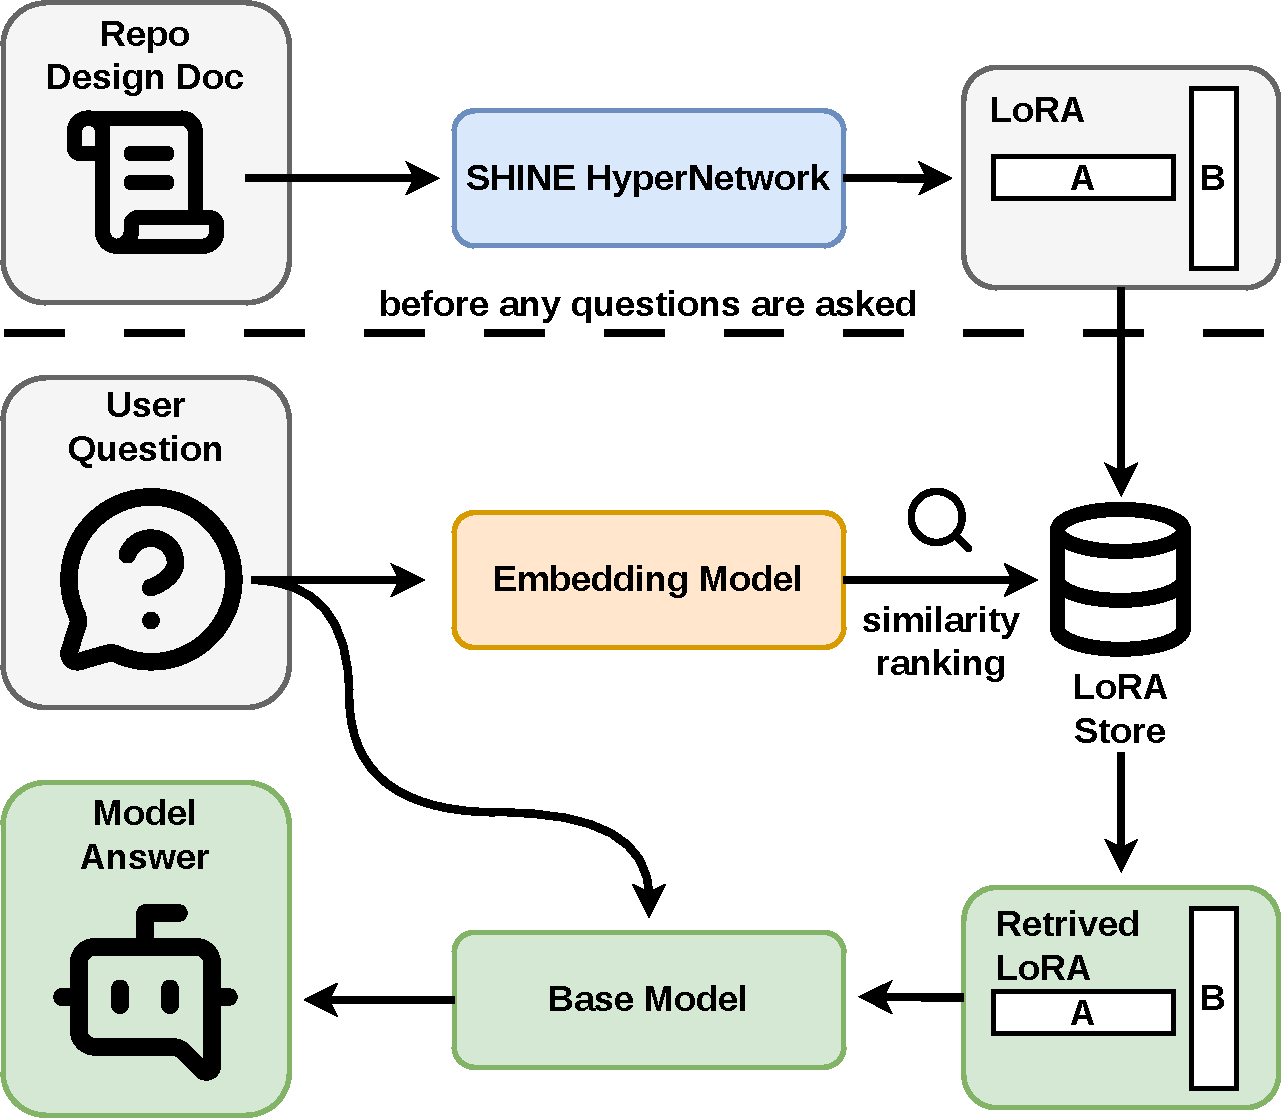
\includegraphics[width=.5\textwidth]{main_design.pdf}
    \caption{Illustration of our question-answering framework. Repository design documents are generated before any question answering and stored. Upon receiving a user question, the question is embedded and its cosine similarity with all stored LoRAs are calculated. The most similar LoRA is then retrieved and loaded into the model, which then gives the answer to the question.}
    \label{fig:shine_flowchart}
\end{figure}

\subsection{Novel Contributions}

MemCoder introduces a novel system for evaluating question answering capabilities of hypernetwork-generated LoRAs used as parametric memory units for code repositories. Prior work has focused on natural language LoRA generation, as well as separate works on LoRA composition and multi-LoRA routing, yet no existing system has created an end-to-end pipeline focused on codebase understanding. 

Rather than utilizing LoRAs in their original use case for SFT, we create modular memory shards encapsulating code repository details from design documents into parametric memory updates. A single SHINE forward pass allows the base model to answer repository questions without having the original document in context, re-framing LoRA as a storage and retrieval tool instead of for PEFT.

Our evaluation reveals that SHINE LoRAs are able to preserve code identifier associations effectively relative to the naïve model, although that gap shrinks when dealing with multi-fact conceptual questions. We also demonstrate that prose-first documents containing minimal backtick density produce meaningfully better LoRAs than documentation that is code-dense. These findings are actionable guidance for researchers continuing to build on hypernetwork-generated adapter infrastructure.

We also provide a reproducible artifact generation pipeline for LoRA-as-memory research. From topic discovery and document generation to SHINE LoRA creation and embedding-based routing, our project provides a fully open-source system that can be integrated with new repositories or LoRA routing and composition methods. Reproduction is easily enabled for both developers and researchers through our versioned prompt templates and JSON schemas, as well as access to pre-generated LoRAs.

\begin{figure}[h]
    \centering
    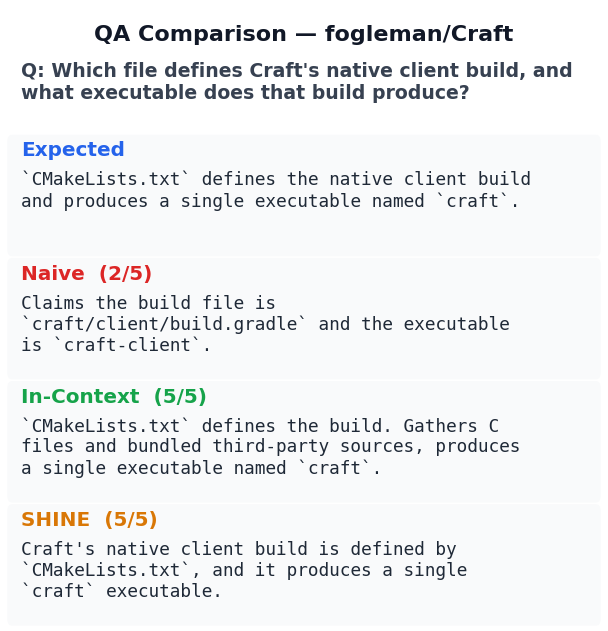
\includegraphics[width=.5\textwidth]{qa_comparison.png}
    \caption{An example repo-specific question and various responses. In the na\"ive environment, the model is given no extra information about the expected answer (in blue), and so it generates vague, generalized responses. The in-context (green) and SHINE (yellow) responses both get ``full credit'' for identifying the specifics of the repo's CMake build system. However, the model using SHINE LoRA weights consumes no extra context tokens to obtain that answer.}
    \label{fig:qa_comparison}
\end{figure}

\subsection{Value \& Availability}

The intended users of this work are developers using LLM-based coding agents that require repository-specific information without divulging details through context tokens or external API calls. MemCoder's pipeline and evaluation harnesses are open source available at \href{https://github.com/sebseager/memcoder}{\texttt{sebseager/memcoder}}. This allows researchers to reproduce results and expand our benchmark to novel repositories. Further, developers can integrate the SHINE LoRA routing infrastructure for question time in their own systems. Given the efficiency around single forward pass LoRA generation, alongside embedding-based routing capable of operating through small locally-runnable models, the system is tailored for privacy-sensitive coding environments where source code remains local with developers. Future work includes migrating all generated documents from Claude Code to be locally generated via Qwen 3-8B or similar models. For researchers aiming to reproduce our experiments, all LoRA artifacts for repositories analyzed in our project are available and allow immediate research without GPU access for LoRA generation.

\section{Background and Motivation}

Modern software engineering (SWE) agents rely on LLMs for codebase questions, identifying relevant files, and implementation standards. However, limited context is often insufficient for large persistent repos. RAG commonly retrieves relevant details, appending them to models' inputs. Work on domain-specific RAG systems via fine-tuning highlights limitations of retrieved text in specialized fields with idiosyncratic terminology~\cite{erakLeveragingFineTunedRetrievalAugmented2024}. Fine-tuned RAG systems show that retrieval alone is often not enough for specialized technical domains, motivating the use of PEFT methods such as LoRA to internalize domain knowledge. Dynamic Parametric RAG (DyPRAG)~\cite{tan2025dynamicparametricretrievalaugmented} extends this idea by replacing retrieved text with dynamically generated parametric knowledge, suggesting that LoRA-style adapters can function as compact, loadable memory units. Work re-framing LoRA adapters as modular knowledge memories has become increasingly popular, treated beyond an adaptation tool but a memory object with capacity, composability for integrating multiple adapters, and routing capabilities~\cite{back2026understandingloraknowledgememory}. This paper finds that routing accuracy in the selection mechanisms for multi-LoRA systems can be a key bottleneck as mis-routing negates modular memory improvements.

For memory-based LoRAs, we explored mechanisms beyond SFT for generation, particularly hypernetworks. Doc-to-LoRA~\cite{charakornDoctoLoRALearningInstantly2026a} proposes a hypernetwork that maps input context into a LoRA instead of placing long documents in prompts or training through gradient descent per context. This allows design document contexts to be internalized by LoRAs for lightweight parametric memory recall. The paper highlights the capacity for these generated LoRAs to answer downstream queries on unseen information even when those details are withheld from context.

\section{Research Questions \& Answers}
\label{sec:rqs}

\begin{figure*}[t]
    \centering
    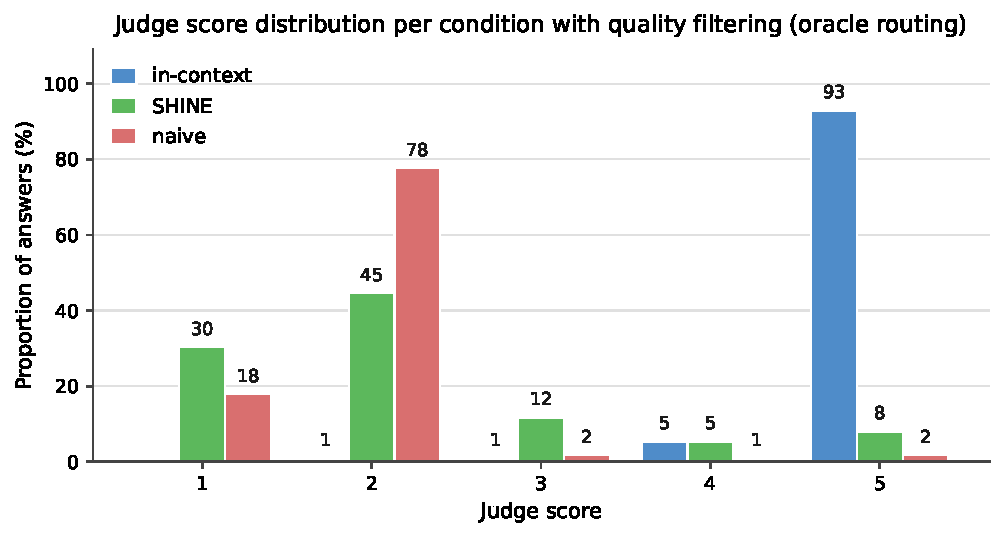
\includegraphics[width=.7\textwidth]{overall.pdf}
    \caption{Performance of our LoRA routing framework (labeled as SHINE) over a quality filtered version $N=112$ of our dataset MemCoder-QA, where questions cannot be accurately guessed without knowledge.}
    \label{fig:overall}
\end{figure*}

\subsection{Can repository-specific knowledge be effectively stored
in small, modular LoRA adapters for code agents?}

Yes, but gains are selective and concentrated on identifier-grounded recall. Across both pilot repositories, stratifying questions by whether the ground-truth answer names a specific code identifier (a backticked token, CamelCase name, or precise value) reveals a sharp asymmetry. On \href{https://github.com/antirez/kilo}{\texttt{antirez/kilo}}, SHINE achieves a mean score
of 3.00 on identifier-targeted questions versus 2.00 for the naïve
baseline (a gap of $+1.00$ on a 5-point scale, roughly $16\times$ the
non-identifier gap ($+0.06$) on the same repository. SHINE also reduces the
'no specifics' failure rate by half on kilo (23\% vs. 47\% for naïve),
meaning the LoRA reliably drives the model to commit to a concrete answer
rather than hedge. On \href{https://github.com/marimo-team/marimo}{\texttt{marimo-team/marimo}}, the directional pattern holds but is weaker. Our results suggest that LoRA-based parametric memory is effective for the retrieval of named entities and specific values, but falls short of in-context prompting for multi-component conceptual questions.
 
\subsection{What is the best unit of organization for parametric
memory?}
 
The original formulation of this research question involved comparing several
candidate input units (subdirectory regions, related file clusters, 
agent-generated design documents) and to examine whether Doc-to-LoRA's
known preference for prose over dense documentation was a property of the
parameterization or the underlying LLM.
 
In practice, the comparison across unit types
was not executed as a controlled experiment; we converged on agent-generated 
prose design documents as the uniform input unit after noticing qualitatively poor 
performance with more complex input schemes. However, our pilot surfaced a
closely related finding: \emph{document style} within a unit type can drive 
LoRA quality. Design documents with high identifier
density (enumerated flag names, struct fields, high backtick density) produced 
LoRAs with visibly degraded outputs (repetition loops, invented identifiers), 
even when those documents were well within SHINE's 1,150-token limit and the 
in-context ceiling remained high. Lean-prose rewrites of two affected kilo 
documents improved mean SHINE scores by $+0.31$ to $+0.70$. 
This is consistent with the style sensitivity
observed in Doc-to-LoRA and suggests the preference for prose is a property
of the hypernetwork parameterization, not solely the base LLM.
A formal comparison of unit types remains future work.
 
\subsection{How should multiple LoRAs be selected and composed at
inference?}

We implemented and evaluated two routing strategies. \emph{Oracle routing}
directly loads the ground-truth LoRA for each question, isolating LoRA
quality from routing quality. \emph{Embedding-based retrieval} embeds each
question and selects the top-$k$ LoRAs by cosine similarity to precomputed
LoRA metadata embeddings; this strategy runs entirely locally using a
small embedding model. A third strategy, Qwen-as-router
(presenting a markdown ledger to Qwen3-8B~\cite{yangQwen3TechnicalReport2025} and asking it to select LoRA
IDs), remains future work.

For $k > 1$, retrieved LoRAs are averaged via rank-concatenation
(\texttt{composition.py}, \texttt{rank\_average}, scale=1.0 by default).
Our embedding routing results are comparable with oracle routing, per Figure~\ref{fig:embedding_routing}. A
controlled ablation of composition quality was not completed due to 
time constraints.

\subsection{How does this approach compare to baselines such as
in-context prompting and RAG, and what are the performance and
efficiency tradeoffs?}

Much of this research question was superseded when we changed 
experimental baselines.
The original baseline plan referenced SWE-Bench Verified and SWE-Bench-CL
as evaluation harnesses. The project pivoted from function-completion on SWE-Bench to a
document-derived QA evaluation formulation, and the baselines changed
accordingly.

The \emph{naïve} baseline (Qwen3-8B with no context and no LoRA)
establishes a floor that is higher than expected: some
doc-derived QA pairs were answerable from pretrained knowledge alone,
inflating the naïve mean score and compressing the naïve--SHINE gap.
Filtering to questions where naïve scored poorly (questions that
actually require the document) gives SHINE a meaningful but not 
decisive advantage. In-context is an upper bound on
what a LoRA compressed from the same document can achieve, and the gap is
large. SHINE reliably matches in-context performance only on single-fact,
identifier-targeted questions with well-written prose documents.
The \emph{RAG-over-design-docs} baseline was not implemented due to 
time constraints. Adding a RAG condition that retrieves the 
top-$k$ most similar documents via the same local sentence
embedder used for LoRA routing is the highest-priority remaining task for
future work.

The original formulation also called for measuring storage cost, adapter
latency, token efficiency, and computational overhead alongside task
performance, using these to characterize whether SHINE's gains justify
its costs. The pivot from SWE-Bench function completion to
document-derived QA changed the setting substantially, and systematic
latency and storage profiling was not instrumented in the evaluation
harness. However, the qualitative tradeoff is clear from the design:
SHINE's LoRA-based approach requires a one-time indexing pass per
document (one SHINE forward pass per LoRA, plus embedding computation)
and loads at most $k$ small LoRA weight dictionaries at query time, with
no document text in the prompt. In-context prompting requires no indexing
but consumes prompt tokens proportional to document length at every
query. A quantitative comparison of these tradeoffs is future work.

\section{Methodology and Metrics}

We propose a harness on Qwen3-8B~\cite{yangQwen3TechnicalReport2025} using the SHINE hypernetwork to construct LoRA adapters from generated repo design documents. At question time, relevant LoRAs are loaded into Qwen3-8B to aid in context-free repository detail recall.

\subsection{Topic Discovery}
The pipeline begins with a target repository compressed into readable design documents from which QA pairs are generated. We first identify a set of collective topics that cover the codebase architecture, dependencies, and functionality. Using a Claude Code agent, the repository's contents spanning READMEs, directory structure, and source files are inspected to generate a set of topics. The prompt to the LLM requires justification of topics with concrete file and directory references from the target repository. Topics fall into two categories, \textbf{(i)} a small universal seed applicable to any repository (e.g., Overview/Purpose, Setup/CLI, Public Interface) and \textbf{(ii)} structure and discovery-derived topics that are codebase specific (e.g., 'Reactive Runtime and Dataflow' for \texttt{marimo} or 'Raw Terminal Input' for \texttt{kilo}). The output is a structured \texttt{topics.json} artifact listing the topic set with evidence-pack hints that guide downstream document generation.

\subsection{Artifact Generation}
We create a structured artifact directory for each target repository. Each directory contains \texttt{repo.json} to record the repository identity and pinned commit, \texttt{topics.json} for storing topic discovery results prior to document generation, and \texttt{ledger.json} to index each \texttt{document\_id} to its corresponding design document, QA pairs, routing examples, embeddings, and generated LoRA paths. An example subdirectory layout is given in Figure~\ref{fig:artifact-structure}. The ledger allows for each document shard to become a candidate for LoRA memory units, allowing downstream tasks to locate relevant source material. This schema ensures proper field completion within design document and question generation tasks necessary for traceability during auditing and evaluation reproduction.


\subsection{Design Documents}
Our pipeline generates a prose design document for each topic of the respective repository. The  document captures pertinent facts, semantic identifiers, or architectural designs, is limited to 1,150 tokens to be within the context limit of the SHINE hypernetwork. Enumeration of flags, constraints, or struct fields is prohibited, as early experimentation found design documents that listed catalog identifiers or utilized bulleted or short-form notation produced LoRA adapters that notably increased unintelligible results and degraded model performance. Some additional style requirements are (i) a backtick budget limiting any backticked terms to a target of 2.5\% with a hard cap at 4\%, (ii) restrictions on quoting code or numeric values, and (iii) verifications of named entities having attached descriptions. Documents are generated by a Claude Code agent following the versioned \texttt{design\_doc\_generation\_v1} prompt and stored as JSON under \texttt{artifacts/<repo>/easy/docs/}.



\subsection{QA Pairs}
Three QA pairs are generated expressly for each design document. QA generation follows the versioned \texttt{doc\_derived\_qa\_generation\_v1} prompt that provides key constraints to mitigate knowledge leakage and ill-formed questions seen in observations of prior experiments and early prompt iterations. For example, questions must explicitly link to definite facts and elements within design documents rather than broad programming queries. Similarly, a self-check step was introduced to ensure questions generated could not be answered by a model without design document context or specific repository training. This restriction aims to mitigate knowledge leakage that was identified in early pilots due to pretrained knowledge of the base Qwen3-8B model about standard, non-repository specific conventions. Further, each QA pair carries metadata including an \texttt{identifier\_targeted} for indicating where correct answers should name a specific code identifier in order for evaluation of syntactical recall versus general conceptual repository  knowledge.

\subsection{SHINE LoRA}
For each design document, SHINE generated a LoRA adapter. The SHINE architecture does a \textit{Memory Extraction} pass where Meta LoRAs augment the frozen LLM to produce memory states, which then feed into a \textit{Parameter Generation} phase where a hypernetwork learns to convert these states into task-specific adapters for inference, as shown in Figure~\ref{fig:shine_architecture}. The hypernetwork architecture utilizes alternating attention across both layer and token dimensions for efficient processing of memory states prior to weight projection, as shown in Figure~\ref{fig:shine_architecture_2}. We use the publicly released SHINE checkpoint (\texttt{checkpoint-epoch-2}) from Hugging Face with a LoRA rank of 8 targeting the FFN down-projection layers. The resulting LoRA weights are saved as .pt files in corresponding repository directories.


This allows our system to generate a LoRA corresponding to each repo design document shard in a single forward pass. This both removes the need for task-specific training with supervised fine-tuning and allows modular loading of adapters at question time via routing. Thus, this step is fundamental to testing our hypothesis for compressing repository context into parametric memory modules via LoRA efficiently to answer questions at inference time without seeing additional repository context.


\subsection{Routing}
At question time, a single LoRA adapter is selected for a given question via oracle or embedding-based routing.

\textbf{Oracle LoRA} returns generated LoRAs corresponding to the specific design document from which the QA pair was derived. As such, this is indicative of a fault-free routing system in which there is no degraded routing accuracy.

\textbf{Embedding-based routing} takes in previously computed embeddings of document retrieval descriptions and the given question using Qwen3-8B and calculates their cosine similarity. The results provide a ranking of candidate LoRAs mapped to each \texttt{qa\_id}, returning top-$k$ LoRA paths at query time.    

\subsection{LoRA Composition}
We utilize rank concatenation with equal weighting to compose multiple LoRA adapters when $k>1$. While a standard $r$-rank LoRA augmented linear layer computes $y=x\cdot W+(x\cdot A)\cdot B$, where $A$ and $B$ are of $\mathbb{R}^{d\times r}$, given $k$ adapters their individual
corrections sum linearly to $\Delta _{\text{combined}} = \sum_{i=1}^{k} (x A_i) B_i$. Thus, producing a single composed adapter with matrices $A'$ and $B'$ from a weighted average of originals is achieved by concatenating A and B matrices along rank dimension and scaling by $\frac{1}{k}$ as shown below 
%
\begin{equation}
A' = \frac{1}{k}\bigl[A_1 \mid A_2 \mid \cdots \mid A_k\bigr], \quad
B' = \begin{bmatrix} B_1 \\ B_2 \\ \vdots \\ B_k \end{bmatrix}
\end{equation}
%
Thus, $(xA')B'$ yields the intended summation $\Delta_{combined}$. 


\subsection{Evaluation Methods}
We compare across three distinct experimental modes for question answering:

\begin{itemize}
    \item \textbf{naïve:} Qwen3-8B is asked the question within a corresponding prompt requesting specific identifiers, steps, or codebase features, without document context or LoRA adapters.
    \item \textbf{In-context:} Qwen3-8B receives the full design document alongside the system prompt to approximate a RAG-style retrieval for answering QA pairs
    \item \textbf{SHINE:} Qwen3-8B receives the question but is augmented with a SHINE-generated LoRA loaded with a routing method. The prompt informs the model it has been adapted to aid in performance in accordance with novel work on model awareness \cite{macar2026mechanismsintrospectiveawareness}. The model is instructed to generate answers using greedy decoding  (\texttt{do\_sample=False}) and without thinking mode \texttt{enable\_thinking=False}). \texttt{<think>} tags and leading 'Final Answer' prefixes are removed prior to scoring. 
\end{itemize}
\subsection{LLM-as-Judge Scoring}
An LLM judge (GPT-5.1) scores answers on a 1 to 5 scale following a versioned rubric (\texttt{llm\_judge\_grading\_v2}). To evaluate the quality of the answer, the LLM judge receives the question, correct answer for reference, model-generated answer, and original design document. The rubric encourages leniency for wording but is harsher on specific identifiers and references to code. To minimize instances observed in prior versions of the versioned rubric where vague yet loosely relevant answers received credit, any responses outside the scope of the design document are treated as fabricated.

A JSON structured response containing the score, descriptive reasoning, and failure tags (\texttt{wrong\_specifics}, \texttt{no\_specifics}, \texttt{missing\_information}, \texttt{off\_topic}, \texttt{refusal\_or\_nonresponse}, \texttt{format\_failure}, and \texttt{other}) is generated. While any score below 5 requires at least one tag, perfect scores clear failure tags. Calls to the LLM use  async concurrency to simultaneously request GPT-5.1 with \texttt{ctx.semaphore} to limit in-flight requests to prevent overwhelming the API. Similarly, exponential backoff is implemented with increasing wait times on successive failures.

\section{Dataset \& Benchmarks}

\textbf{MemCoder-QA (generated).}  We constructed a bespoke evaluation
benchmark of document-derived QA pairs for each target repository.  For
each design document, a prompted LLM agent produced three QA pairs whose
answers are explicitly grounded in that document, accompanied by a
self-check step designed to filter questions answerable from pretrained
knowledge alone.  Each QA record carries metadata fields: document ID,
topic, difficulty, an \texttt{identifier\_targeted} flag (true when the
correct answer names a specific code identifier), and a
\texttt{prompt\_version} for provenance.
The current benchmark spans five repositories at the easy difficulty
tier. Two repos were integrated early for pilot experimentation: \texttt{antirez/kilo} with 3 documents and 43 QA pairs (9 scored
as identifier-targeted), and \texttt{marimo-team/marimo} with 8 documents
and 24 QA pairs (3 scored as identifier-targeted).  Additionally, we added 3 more repos once we completed a final LLM-judge design: \texttt{fogleman\_\_Craft}, \texttt{psf\_requests}, and \texttt{pytest-dev\_pytest}. This brings the design document total to 37, with 136 QA pairs derived from those documents.

QA pairs are stored
as JSON under \texttt{artifacts/<repo>/easy/qas/} and governed by
\texttt{schemas/qa\_pairs.schema.json}.
A separate set of ledger example questions (3–5 per document) was
generated from the same documents under a distinct prompt with explicit
instructions to produce questions different from the evaluation set,
preventing router contamination of the test set.  These appear in
\texttt{artifacts/<repo>/easy/qa\_examples/} and are not used for
evaluation.
Design documents for each repository were generated by a Claude Code 
agent following the versioned \texttt{design\_doc\_generation\_v1} prompt.
Each document is capped at 1,150 tokens (SHINE's context limit), with 
topics spanning Overview/Purpose, Setup, and domain-specific subjects 
discovered by inspecting README sections, top-level directory structure, 
and source files.
Documents are stored as JSON under \texttt{artifacts/<repo>/easy/docs/}
and governed by \texttt{schemas/design\_doc.schema.json}.


\section{Results \& Findings}
\label{sec:results}

We evaluate the performance of our framework over five repositories with 37 design documents in total with 136 question-answer pairs derived from those documents. For each question, we label whether it targets some identifier in the codebase for the question, accounting for $40/136$ of the questions, e.g. Q: ``Which file defines Craft's native client build?'', A:`CMakeLists.txt' (see Fig.~\ref{fig:qa_comparison}). We filter out 24 questions that can be accurately guessed based simply on the text in the question itself to create a quality filtered subset. Figure~\ref{fig:overall} shows the performance of SHINE over these filtered 112 questions. In general, we observe that SHINE out-performs naive but far under-performs in-context performance, where the ground-truth document is included in the context. All judge scores come from GPT-5.1.

\subsection{SHINE performs best on entity recall questions}
Figure~\ref{fig:identifier-targeted} shows performance over all the 136 questions per repository, split by questions labeled as identifier-targeted and other. As we can see, SHINE performs better for four out of the five repositories when answering identifier-targeting questions. This indicates questions focused on nomenclature or value locations are better suited for SHINE than conceptual relationships between variables, highlighting the limits of knowledge transferred via LoRAs.

\begin{figure}[h]
    \centering
    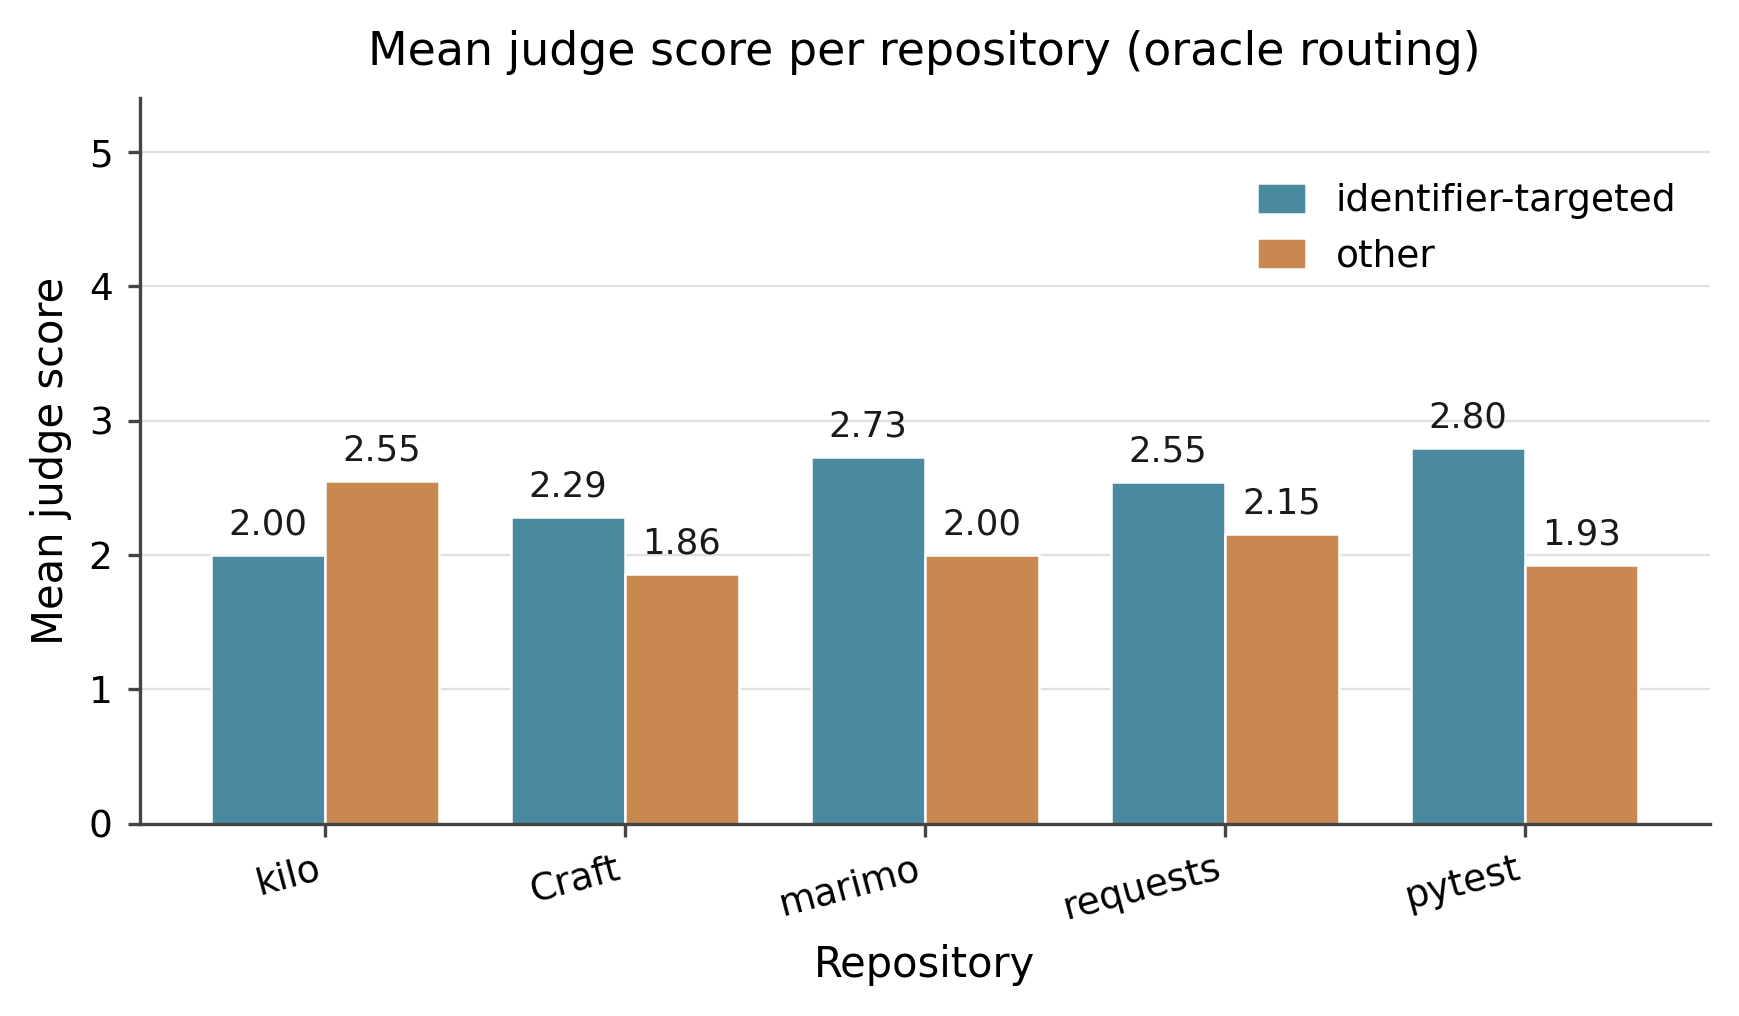
\includegraphics[width=.5\textwidth]{oracle_identifier-targeted.png}
    \caption{The mean judge score per repository SHINE with oracle routing, split between question which test recall of named symbols (labeled identifier-targeted) and the other questions.}
    \label{fig:identifier-targeted}
\end{figure}


\subsection{SHINE LoRA composition can preserve signal but does not significantly improve recall}

We evaluated whether multiple document-specific LoRAs can be combined into a single adapter, and whether doing so would allow the model to ``learn'' the set of information contained in all the source documents. We used the \texttt{kilo} repository and composed three LoRAs corresponding to the overview, terminal input, and editing/persistence documents. The composed adapter is formed by rank-averaging the three LoRA updates, and we compared it against each individual document LoRA. Unless otherwise noted, assume that we are using the oracle routing method as an upper-bound on performance instead of the embedding model routing.

Figure~\ref{fig:combined_qa} shows that composition performs comparably to the strongest individual adapters, but does not clearly improve over them. The composed adapter achieves a mean judge score of $2.51$ over $49$ judged rows, compared with $2.55$ for the overview LoRA, $2.45$ for the terminal input LoRA, and $2.05$ for the editing/persistence LoRA. This suggests that rank-averaged composition preserves some useful document knowledge, but the benefit is limited: the composed adapter does not reliably integrate the three sources into a stronger unified representation. Instead, composition appears to behave like a lossy blend of the individual LoRAs, retaining enough signal to remain competitive but not enough to close the gap to in-context retrieval.

\begin{figure}[h]
    \centering
    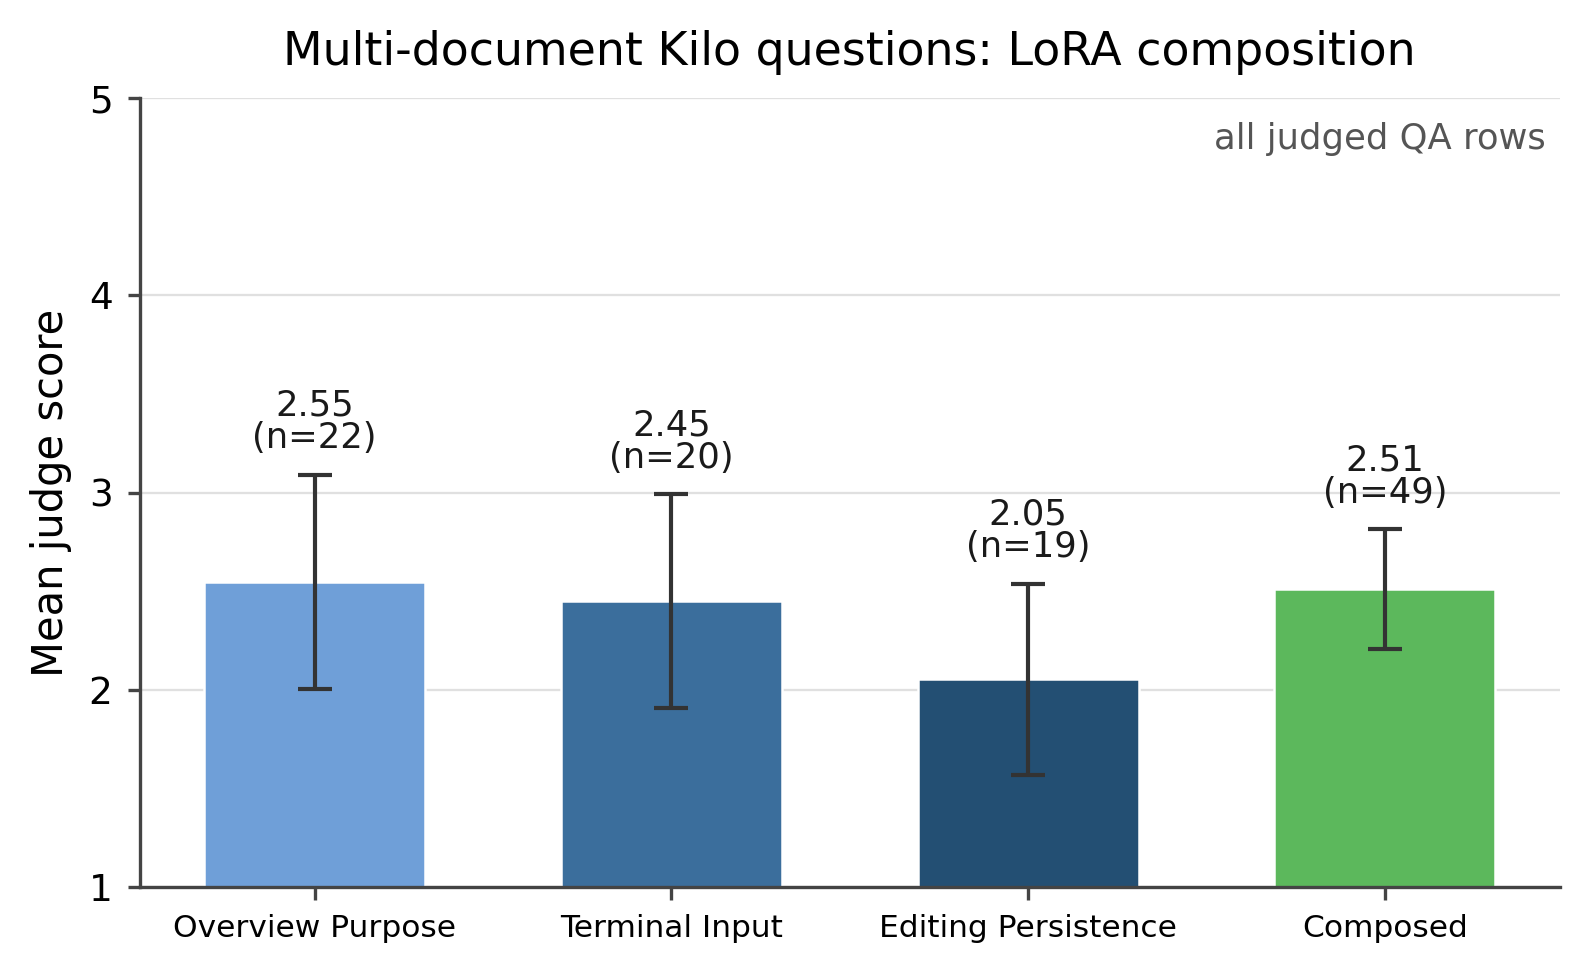
\includegraphics[width=.5\textwidth]{combined_qa_judge.png}
    \caption{Mean LLM judge score on multi-document Kilo questions requiring LoRA composition. The composed adapter averages the three document-specific LoRAs and is compared against each individual LoRA used alone. Scores are on a 1--5 scale; higher is better.}
    \label{fig:combined_qa}
\end{figure}

When restricting the analysis to only questions that require multiple source documents, composition becomes more favorable but remains weak overall. On this subset, the composed adapter reaches a mean judge score of $1.83$ across $6$ questions, compared with $1.17$, $1.67$, and $1.50$ for the three individual LoRAs. Although this filtered sample set (as available at time of writing) is likely too small to be able to draw meaningful conclusions, the experiment suggests that composition does recover some cross-document signal. However, the low absolute score shows that simple rank-averaging is still insufficient for reliable multi-document reasoning: it improves over isolated LoRAs but does not successfully synthesize the combined evidence needed to answer these questions well.


% \subsection{SHINE maintains associations between identifiers over general document content}

% Segmenting questions based on whether their ground-truth answer includes a code identifiers, such as backticked tokens or camelCase names, highlights a discrepancy in SHINE's effectiveness, as seen in Table~\ref{tab:identifier-stratification}. The gap between naïve and SHINE performance on identifier-targeted ($+1.00$) is roughly $16\times$ larger than for non-identifier questions ($+0.06$). Questions focused on nomenclature or value locations are better suited for SHINE than conceptual relationships between variables. This observation holds true across repositories. For \texttt{marimo}, the identifier-targeted gap ($+0.33$) similarly exceeds non-identifier ($-0.05$). However, there are only 3 qualifying questions in this bucket, warranting further studies for more conclusive inter-repository generalizations.

\subsection{SHINE Achieves Perfect Scores Only on Single-Fact Ground Truths}
 
\begin{table}[h]
\centering
\caption{Rate of high SHINE scores by repository.}
\label{tab:score-ceiling}
\begin{tabular}{lcc}
\toprule
\textbf{Repo} & \textbf{SHINE score $\geq 4$ (n)} & \textbf{of which 5s} \\
\midrule
kilo     & 11/43 (25.6\%) & 5 \\
Craft    & 2/21  (9.5\%)  & 1 \\
marimo   & 4/24  (16.7\%) & 3 \\
requests & 5/24  (20.8\%) & 3 \\
pytest   & 4/24  (16.7\%) & 2 \\
\midrule
\textbf{Total} & \textbf{26/136 (19.1\%)} & \textbf{14} \\
\bottomrule
\end{tabular}
\end{table}

As can be seen in Table~\ref{tab:score-ceiling}, SHINE is capable of producing high scoring answers. Half of all responses scoring 5 are questions labeled identifier-targeting, highlighting that SHINE performs best when requiring targeted look up as opposed to conceptual understanding. LoRAs compress well named symbols but struggles compressing multi-step procedures. Here are two example questions from kilo that SHINE scored perfectly on:
\begin{enumerate}
    \item Q:``How is kilo invoked?'' $\rightarrow$ A:``\texttt{kilo <filename>}''
    \item Q:``Which global structure holds editor state?'' $\rightarrow$ A:``\texttt{struct editorConfig}''
\end{enumerate}

\subsection{SHINE improves confidence around specifics recall}
The rubric splits \texttt{missing\_information} failure-mode tag into \texttt{no\_specifics} (answer lacking ground-truth facts) and \texttt{missing\_information} (answer commits to specifics but lacks required ones).

\begin{table}[h]
\centering
\caption{Failure-mode rates under the v1 rubric by condition.}
\label{tab:failure-modes}
\begin{tabular}{llcc}
\toprule
\textbf{Repo} & \textbf{Condition} & \texttt{no\_specifics} & \texttt{wrong\_specifics} \\
\midrule
marimo & naïve & 62\% & 46\% \\
marimo & SHINE & 46\% & 42\% \\
kilo   & naïve & 47\% & 53\% \\
kilo   & SHINE & \textbf{23\%} & 49\% \\
\bottomrule
\end{tabular}
\end{table}

The SHINE for kilo has half the rate of \texttt{no\_specifics} compared to kilo naïve (23\% vs.\ 47\%), while roughly a similar \texttt{wrong\_specifics} rate. This suggests the LoRA encourages model commitment to a concrete answer over tending towards generic responses characteristic of the naïve model.

\subsection{Question-Style Sensitivity}

\texttt{marimo} results by source document demonstrate a sharp deviation in SHINE performance as document type varies. 

\begin{table}[h]
\centering
\caption{Per-document SHINE vs.\ naïve gaps on \texttt{marimo} (v1 rubric, sorted by gap).}
\label{tab:per-doc-marimo}
\begin{tabular}{lccc}
\toprule
\textbf{Document} & \textbf{naïve} & \textbf{SHINE} & \textbf{Gap} \\
\midrule
\texttt{sql\_data\_integrations\_1}       & 2.00 & 3.00 & \textbf{+1.00} \\
\texttt{reactive\_runtime\_dataflow\_1}   & 1.67 & 2.67 & \textbf{+1.00} \\
\texttt{setup\_cli\_1}                    & 1.33 & 2.00 & +0.67 \\
\texttt{public\_interface\_1}             & 2.33 & 2.67 & +0.33 \\
\texttt{apps\_scripts\_wasm\_1}           & 2.00 & 1.67 & $-$0.33 \\
\texttt{ai\_mcp\_pairing\_1}              & 1.67 & 1.33 & $-$0.33 \\
\texttt{overview\_purpose\_1}             & 2.00 & 1.33 & $-$0.67 \\
\texttt{ui\_outputs\_interactivity\_1}    & \textbf{3.33} & \textbf{1.67} & \textbf{$-$1.67} \\
\bottomrule
\end{tabular}
\end{table}

SHINE performance is worst for \texttt{ui\_outputs\_interactivity\_1}, containing a meaningful density of concepts alongside QA pairs with multi-fact reasoning questions, such as \textit{'Why does marimo require an interacted UI element to be bound to a global variable for notebook reactivity?'}. naïve provides a plausible summarization to earn partial credit; SHINE suffers complete topic drift, however. SHINE performance improves for documents naming concrete mechanisms ((\texttt{sql\_data\_integrations}, \texttt{reactive\_runtime\_dataflow})), yet fails to maintain performance where those mechanisms require deeper explanation. 

\subsection{Repository Profile Impacts LoRA Effectiveness}

\begin{table}[h]
\centering
\caption{Repository-level comparison of SHINE amenability.}
\label{tab:repo-profile}
\begin{tabular}{lcc}
\toprule
& \textbf{marimo} & \textbf{kilo} \\
\midrule
Mean words/doc               & 625   & 538   \\
Mean identifiers/doc         & 3.8   & 10.7  \\
\% answers naming identifier & 12.5\% & 23\% \\
naïve baseline (v1)          & 2.04  & 2.37  \\
SHINE baseline (v1)          & 2.04  & \textbf{2.65} \\
SHINE--naïve gap             & 0.00  & \textbf{+0.28} \\
\bottomrule
\end{tabular}
\end{table}

Design documents for \texttt{kilo} contain $3\times $ more identifiers with $2\times$ rate of identifier-targeted QA pairs. For $\texttt{marimo}$, the SHINE vs. naïve gap is $0.00$ but slightly positive ($+0.28$) for $\texttt{kilo},$ suggesting the smaller codebases containing purpose-built modules and high identifier density in design documents are conditions for SHINE outperformance. 




\subsection{Prompt Engineering Variations}
Different system prompts were tested for the question answering model, the results of which are displayed in Table~\ref{tab:prompt-gap}. One failure mode we noticed was that the responses from the SHINE method were too short, so we modified the prompt to encourage adding necessary detail to answer a question fully and observed a performance boost (labeled ``detail'' in the table). We then mirrored this system prompt for also the naive and in-context conditions. Further, we observed that the SHINE model performs best if we added a sentence telling the model that it had been adapted with the necessary information (labeled ``adapted'' in the table). This is a very interesting finding, which invites follow-on work. The system prompt for the SHINE model is the following:
\begin{quote}
``Your weights have been adapted to encode a specific document about a code repository. Draw on that adapted knowledge to answer. You are a helpful assistant. Answer with specific detail — name the identifiers, mechanisms, or steps the question is asking about. If the question asks for  multiple items, list each one.''
\end{quote}

\begin{table}[h]
\centering
\caption{SHINE--naïve gap under different system prompts.}
\label{tab:prompt-gap}
\begin{tabular}{lcc}
\toprule
\textbf{Prompt} & \textbf{marimo gap} & \textbf{kilo gap} \\
\midrule
baseline & +0.00 & +0.28 \\
detail   & +0.17 & +0.60 \\
adapted  & +0.26 & +0.65 \\
\bottomrule
\end{tabular}
\end{table}

\section{Ablation Study}

To evaluate the effectiveness of the embedding-based LoRA routing mechanism, we ran an ablation experiment across five repositories to determine the gap between our routing pipeline and an oracle LoRA baseline. Results are shown in Figure~\ref{fig:embedding_routing}.
 


\begin{figure}[h]
    \centering
    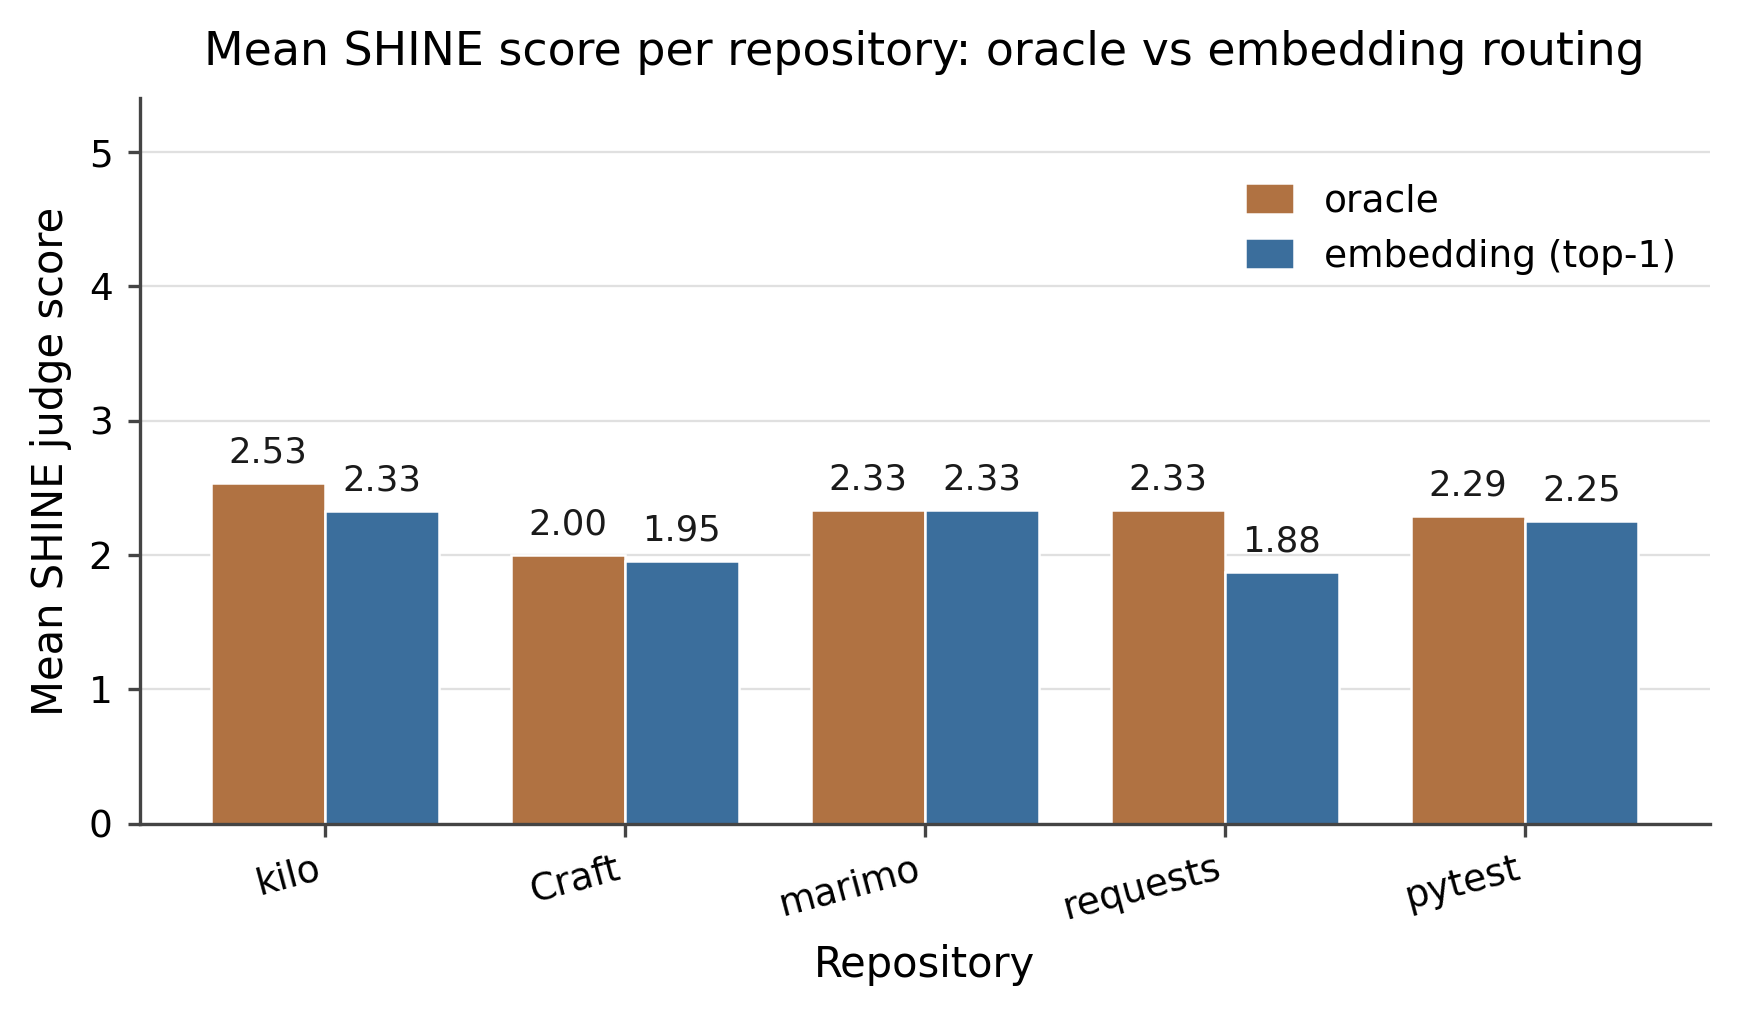
\includegraphics[width=.4\textwidth]{oracle_v_embedding_per_repo.png}
    \caption{Mean judge score per repository evaluated on, comparing between the oracle and embedding routing methods.}
    \label{fig:embedding_routing}
\end{figure}

As expected, oracle routing outperforms embedding routing in four of five repositories, matching performance in one. The overall mean degradation is $-0.15$, demonstrating near ideal performance from the top-1 embedding mechanism. The gap notably varies by repository, with  \texttt{requests} showing the greatest drop of $-0.45$, suggesting the LoRA metadata embeddings are less correlated with the QA pairs. Conversely,  \texttt{marimo} shows zero degradation as the embedding router reliably selects the LoRA best suited for the QA pair. Other repositories show minimal loss and suggest codebases with well-separated topics allow for embedding-based routing to be near ideal.

These data points provide insight into the capabilities of routing, which while naturally subpar to oracle LoRAs, can at times be sufficient when perfect selection is unavailable. Future work can include improved embedding models coinciding with richer metadata for LoRA descriptions and artifacts.

\section{Conclusion}

We demonstrate that LoRAs are successful tools for distilling repository knowledge in small, local coding agents. We augment existing work for transforming documents into LoRAs with a framework for extracting repository information, carefully generating LoRAs from this extracted information, and storing and retrieving these LoRAs automatically at run-time. We find that the LoRAs best compress information relating to named symbol recall and struggle more with compressing multi-step procedures related to a repository. 

Furthermore, we find that a lightweight embedding model ranking candidate LoRAs by cosine similarity performs nearly as well as choosing the best LoRA for a given question.
Our experiments show that a common failure mode is that the adapted models respond overly tersely, which remains stubborn even experimenting with various system prompts. Though we do find improved performance when informing the model that it has been adapted, which encourages further research into the capability of model introspection of adapted knowledge. We additionally find that LoRA composition does not lead to significant performance loss.

Given security and privacy issues of feeding private codebases to frontier lab APIs, we provide this framework as a way of increasing the repository knowledge in small, locally hosted models.
\section{What Was Delivered \& Where Is It?}

All code, scripts, prompts, schemas, generated artifacts, evaluation
results, and documentation are available on GitHub at
\href{https://github.com/sebseager/memcoder}{\texttt{sebseager/memcoder}}.
The repository is organized as follows.
The \textbf{evaluation harness} lives under \texttt{eval/} with 
its CLI at \texttt{scripts/run\_eval.py}.  It accepts a
self-contained YAML config and exposes four subcommands:
\texttt{predict} (Qwen3-8B inference with optional LoRA), \texttt{judge}
(OpenAI \texttt{gpt-5.1} LLM-as-judge), \texttt{report} (per-condition
aggregation and plots), and \texttt{all} (full pipeline).  Every
invocation writes a timestamped results directory containing 
\texttt{predictions.jsonl}, \texttt{judgments.jsonl},
\texttt{report.md}, and various plot files.
\textbf{Artifact pipeline scripts} under \texttt{scripts/} include
\texttt{generate\_shine\_lora.py} (bake one SHINE LoRA from a given 
design document and update the ledger), \texttt{embedding\_router.py}
(precompute embedding-based routing results), and
\texttt{validate\_artifacts.py} (check JSON artifacts against schemas).
Analysis utilities (\texttt{plot\_naïve\_hard.py},
\texttt{prompt\_ab\_test.py}, \texttt{rubric\_impact.py}, and others)
process judged run directories and produce the stratified tables reported
in Section~\ref{sec:results}.
\textbf{Versioned prompt templates} under \texttt{prompts/} cover topic
discovery (v1), design-document generation (v1), doc-derived QA
generation (v1 and v2), ledger example-question generation (v1), and
LLM-judge rubrics (v0, v1, v2; current default v2).  Each template
carries an explicit version string that generated artifacts record in
their metadata.
\textbf{JSON schemas} under \texttt{schemas/} define the various 
artifact contracts for easy validation in scripts.
Generated \textbf{artifacts} under \texttt{artifacts/} include
easy-tier design documents, question-answer pairs, pre-baked LoRA \texttt{.pt}
dictionaries, and ledger files for all five target repositories: \texttt{fogleman\_\_Craft},
\texttt{psf\_\_requests}, \texttt{pytest-dev\_\_pytest},
\texttt{antirez\_\_kilo}, and \texttt{marimo-team\_\_marimo}).
An interactive Streamlit inspection dashboard (as presented during the 
in-class demo) under \texttt{dashboard/} supports artifact browsing, 
LoRA-answer inspection, routing exploration, and result analysis.


\section{External Materials}

The background situates MemCoder relative to several existing approaches:
retrieval-augmented generation~\cite{lewis2021retrievalaugmentedgenerationknowledgeintensivenlp},
parameter-efficient fine-tuning (LoRA)~\cite{hu2021loralowrankadaptationlarge},
DyPRAG-style dynamic parametric memory~\cite{tan2025dynamicparametricretrievalaugmented}, and the
understanding of LoRAs as modular knowledge memories~\cite{back2026understandingloraknowledgememory}.

The main external component for the current version of our experiment 
is Scalable Hyper In-Context Network (SHINE)~\cite{liuSHINEScalableInContext2026},
which maps an input context into a LoRA adapter in a single forward pass.
We use SHINE checkpoints made available by the original authors without 
additional training, findable at their repo: \href{https://github.com/MuLabPKU/SHINE}{\texttt{MuLabPKU/SHINE}}.
Our work's contribution is the evaluation setting, artifact pipeline, and 
routing infrastructure layered on top of it.
The SHINE checkpoint used is \href{https://huggingface.co/papers/2602.06358}{\texttt{checkpoint-epoch-2}}, published by the vendor on Hugging Face and obtained via \texttt{scripts/download\_checkpoints.sh}.
The frozen base model for all prediction conditions was the 
\textbf{Qwen3-8B} variant~\cite{yangQwen3TechnicalReport2025}. 
It serves as the backbone for SHINE's 
hypernetwork and the evaluated model under all three conditions 
(naïve, in-context, SHINE). No fine-tuning of Qwen3-8B was performed.
\textbf{OpenAI gpt-5.1} was used exclusively as the LLM-as-judge.  The
judge receives the question, ground-truth answer, model answer, and the source design document, and emits a structured
1-5 correctness score with failure-mode tags.  It has no role in
indexing or answering.
Embedding-based routing can use any small embedder. In our testing, 
we used \texttt{Qwen/Qwen3-Embedding-0.6B} to embed both LoRA metadata 
and user questions.
Five repositories are fully evaluated. Two example repositories are given below:
\texttt{antirez/kilo}~\cite{sanfilippoAntirezKilo2026}, a $\sim$1,000-line single-file C text
editor, and \texttt{marimo-team/marimo}~\cite{agrawalMarimoOpensourceReactive2023}, a Python reactive
notebook framework substantially larger in scope.  All are open-source
projects and publicly available on GitHub.


\section{Reproducibility}

The evaluation harness is fully deterministic given fixed model weights and
pre-baked LoRA files.  Each results directory contains a
\texttt{run\_config.yaml} and \texttt{manifest.json} recording the git
SHA, model paths, prompt file paths, and per-artifact input records,
sufficient to reproduce any single judged row from
\texttt{predictions.jsonl} without re-running the full pipeline.
Hardware requirements are a CUDA-capable GPU (e.g., A6000, 48GB VRAM) 
sufficient to load Qwen3-8B in inference mode.
SHINE's (\texttt{checkpoint-epoch-2}) is downloaded from Hugging Face 
and used unmodified. Judge calls require an \texttt{OPENAI\_API\_KEY} 
with access to \texttt{gpt-5.1}; this is the only external network call 
in the pipeline.  All other components run fully locally with no external 
API calls.
 
The artifact pipeline (topic discovery, document generation, QA
generation) uses Claude Code or a comparable frontier coding agent under
versioned prompts.  Generated artifacts record their \texttt{prompt\_version}
and generator identity in JSON metadata.  Re-running the artifact
pipeline from scratch will produce semantically similar but \textit{not}
bit-for-bit identical artifacts due to LLM temperature.  The evaluation
pipeline (predict, judge, report) is fully reproducible from the
pre-baked artifacts already in the repository.

Because we rely on LLM-as-judge, judgments made by (\texttt{gpt-5.1}) may
exhibit run-to-run drift. We mitigate by logging the judge's full
\texttt{reasoning} and \texttt{raw\_response} fields in
\texttt{judgments.jsonl} for spot-checking. A recommended step to 
validate judge performance is hand-grading of a calibration set of 
30-50 questions.



\section{Who Did What}
 
\textbf{Brian Siegel:} I designed, implemented, and helped evaluate the LoRA routing component and the methods of selecting ideal LoRAs at inference time. I first helped to adapt artifacts and the repository structure to work within a ledger-based pipeline. I helped build the architecture for the \texttt{ledger.json} that bridges the paths between design documents, QA pairs, LoRA artifacts, and the routing mechanism. I implemented the embedding-based LoRA router using Qwen 3-8B to create a ranked top-k list of SHINE LoRAs based on the cosine similarity between the question embedding and LoRA candidate profile. I debugged issues around truncation of long inputs to coincide with smaller models context windows length, ledger parsing, and subsequently ran experiments with small embedding models such as $\texttt{infloat/e5-small-v2}$ for early pilot runs. I evaluated routing accuracy on the repositories, and additionally generated and validated an additional set of QA pairs from the \texttt{antirez/linenoise} repository for preliminary top-k routing ablation across design documents. 
Additionally, I built out the evaluation harness for testing routed LoRA answers beyond routing accuracy when compared to oracle LoRAs. The separate \texttt{run\_routed\_lora\_eval.py} harness integrated with the original LoRA evaluation script to experiment between individual oracle LoRA adapters, an all-LoRA composition baseline, the top-k embedding router, and static, design document-specific LoRAs. I added JSONL file loading support, mapped between QA pairs and routed LoRA IDs, and computed routed against non-routed performance. I also aided in many of the prior pilot experimentations before settling on SHINE for QA, particularly debugging and running experiments on a prior task of training SHINE LoRAs on function completion and creating a bespoke dataset of masked SWE-Bench code.
 
\textbf{Seb Seager:} I implemented early work into alternative approaches before the team settled on SHINE, including attempts to build on Doc-to-LoRA and DyPRAG, and an effort to train oracle LoRAs directly on the QA task as a hypernetwork benchmark. None of these panned out, but informed the direction the project eventually took (and are now archived in the \texttt{old} directory). I identified the SHINE method, reproduced the results from the paper, and set up initial code for integrating SHINE into our testing pipeline. I wrote scripts for generating LoRAs from source documents using the SHINE hypernetwork, and contributed to the JSON schema architecture and pieces of the validation harness. I ran iterative experiments on Columbia's Insomnia HPC cluster to collect test data and interpreted results across pilot runs. I also built the interactive dashboard used to demo the framework's performance.

\textbf{Magnus Saebo:} I came up with the original plan for the project, and devised the new direction after feature implementation was found to be infeasible to teach through LoRAs, then deciding to pivot to repository question-answering. I built out the evaluation pipeline, whereby someone would give a model, an embedding model, and a hypernetwork, and evaluate this triple over the set of questions. I did not do the embedding routing, but rather the architecture that it folded into. I also was largely responsible for picking which repositories we evaluated against, and I was responsible for scraping all the relevant data from those repositories: the design documents, the question-answer pairs, and the other information placed in the ledger. I designed the experiment comparing the oracle and embedding routing experiment as well as the overall performance comparison between SHINE, in-context, and naive.
 
 
\section{What We Learned}
 
\textbf{Brian Siegel:} One of the most unexpected lessons was the amount of time instantiating the backend infrastructure for model inference takes. Running models across environments, both Columbia's HPC cluster as well as local machine jobs via Ollama and vLLM-Metal, were consistently challenging. Various environments contained unique obstacles, whether learning how to navigate disk quotas on the HPC, mismatched flash-attention wheels leading to patching vendor code, or Qwen 3-8B token over-consumption due to thinking mode. This taught me to start with simplistic evaluations at first before scaling. Prior to vLLM serving, it may have been best to ensure one QA pair was answered successfully in one configuration and then add complexity once verified.

I also gained a greater understanding of the LoRA mechanism beyond its fine-tuning applications. Working with cosine similarities and hypernetwork architectures provided meaningful insight into the mathematical and theoretical principles that allow adapters to function as parametric memory updates. 


 
\textbf{Seb Seager:} Compression of natural context into LoRAs is more lossy than I had expected. It makes some sense, given that most LoRA research emphasizes semantic understanding, not precise and reliable recall, but this was an especially tricky hurdle in a LoRA-for-codebases project. In a similar vein, trying to compress large amounts of information into a LoRA---or trying to compose many unrelated LoRAs---is likely going to be unhelpful. When dealing with training models, or even doing inference on large datasets, small pilot runs to validate signal before scaling is important. It's easy to pick ``good enough'' decision gate tolerances after the fact, but choosing thresholds first is more informative.
 
\textbf{Magnus Saebo:} We learned that it is best not to have a fixed plan, and that it is very necessary to adapt plans based on the results. We started with very lofty goals for the paper, imagining using LoRAs for adapting a model to more successfully perform issue-resolution tasks, a la SWE-Bench, but quickly found that LoRAs at rank 8 would not be sufficient without much greater finetuning of the hypernetworks used. Additionally, we learned to get results quickly instead of planning out deeply in hypotheticals. Our original plan doing issue-resolution involved folding in findings from the continual learning literature, and we spent time thinking through how this might happen. Though our ambitions would be lowered as soon as we actually tried to get these LoRAs to encode sufficiently complex information. Instead of hypothesizing further and further, we learned the value of doing toy experiments first to understand the limitations of the methods we have to work with.




\section{Bibliography}

\printbibliography

\section{Appendix}

\subsection{Artifact directory structure for \texttt{antirez/kilo}}

\begin{figure}[H]
\centering
\begin{minipage}{0.8\linewidth}
\begin{verbatim}
artifacts/
  antirez__kilo/
    repo.json
    topics.json
    ledger.json
    easy/
      docs/
      qas/
      qa_examples/
      loras/
    eval_results.jsonl
\end{verbatim}
\end{minipage}
\label{fig:artifact-structure}
\end{figure}

%\subsection{Identifier sensitivity study}

%\begin{table}[H]
%\centering
%\caption{SHINE vs. naïve performance stratified by whether the ground-truth answer names a specific code identifier}
%\label{tab:identifier-stratification}
%\begin{tabular}{llcccc}
%\toprule
%\textbf{Repo} & \textbf{Stratum} & \textbf{n} & \textbf{naïve} & \textbf{SHINE} & \textbf{Gap} \\
%\midrule
%marimo & identifier-targeted & 3  & 2.00 & 2.33          & +0.33          \\
%marimo & non-identifier      & 21 & 2.05 & 2.00          & $-$0.05        \\
%kilo   & identifier-targeted & 10 & 2.00 & \textbf{3.00} & \textbf{+1.00} \\
%kilo   & non-identifier      & 33 & 2.48 & 2.55          & +0.06          \\
%\bottomrule
%\end{tabular}
%\end{table}

\subsection{SHINE architecture overview}

\begin{figure}[H]
    \centering
    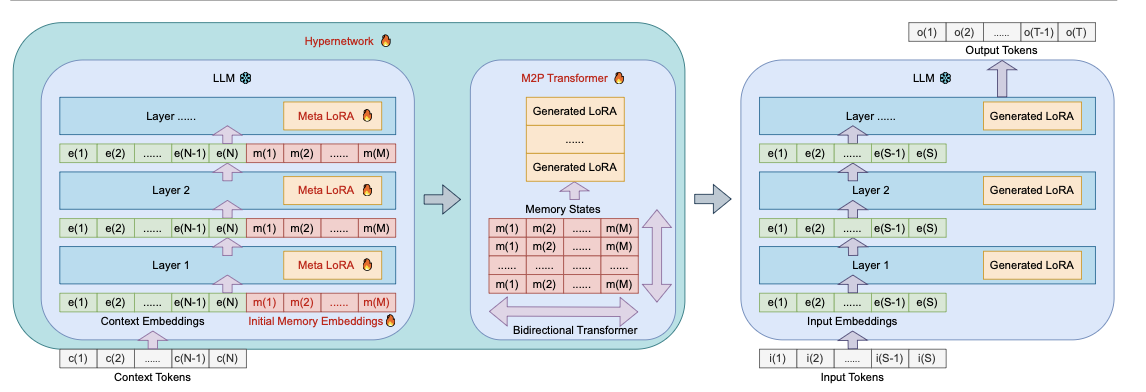
\includegraphics[width=\linewidth]{shine1.png}
    \caption{Overview of the SHINE training architecture. SHINE maps an input context into generated LoRA adapters in a single forward pass, allowing the downstream LLM to answer context-dependent questions without directly including the original context in the prompt.}
    \label{fig:shine_architecture}
\end{figure}

\begin{figure}[H]
    \centering
    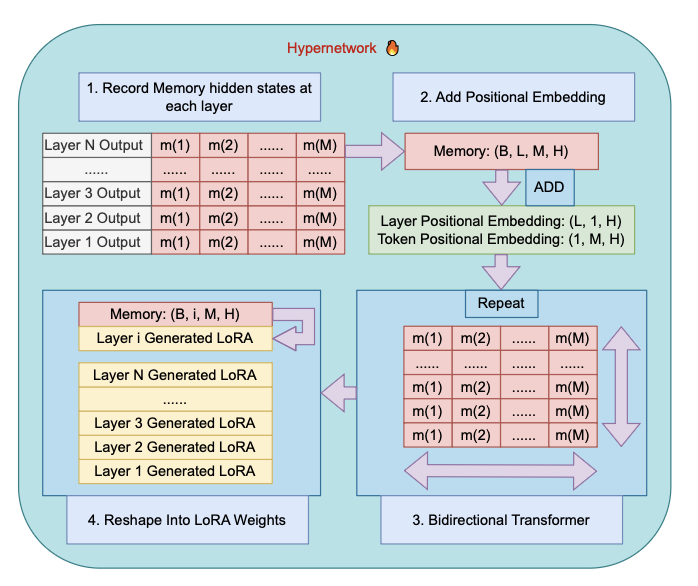
\includegraphics[scale=0.8]{shine2.png}
    \caption{Detailed breakdown of SHINE hypernetwork architecture. SHINE records memory hidden states for each layer along with positional tokens, and reshapes the memory states into LoRA weights with a bidirectional transformer.}
    \label{fig:shine_architecture_2}
\end{figure}

\end{document}
